\chapter{数学模型}\label{cha:model}
\section[非协作定位场景]{非协作定位场景}\label{section:noncooperative_localization}

        考虑一个平面定位场景中部署了$N_b$个位置已知的\textbf{锚点},锚点的位置记为$\{\bm{p}^b_1,\bm{p}^b_2,...\bm{p}^b_{N_b}\}$,现在要对场景中一个\textbf{位置未知}的节点进行定位,待定位节点的位置为$\bm{p}$,如图(\ref{fig:non_cooperative_spatial})所示。
        \begin{figure}
          \centering
        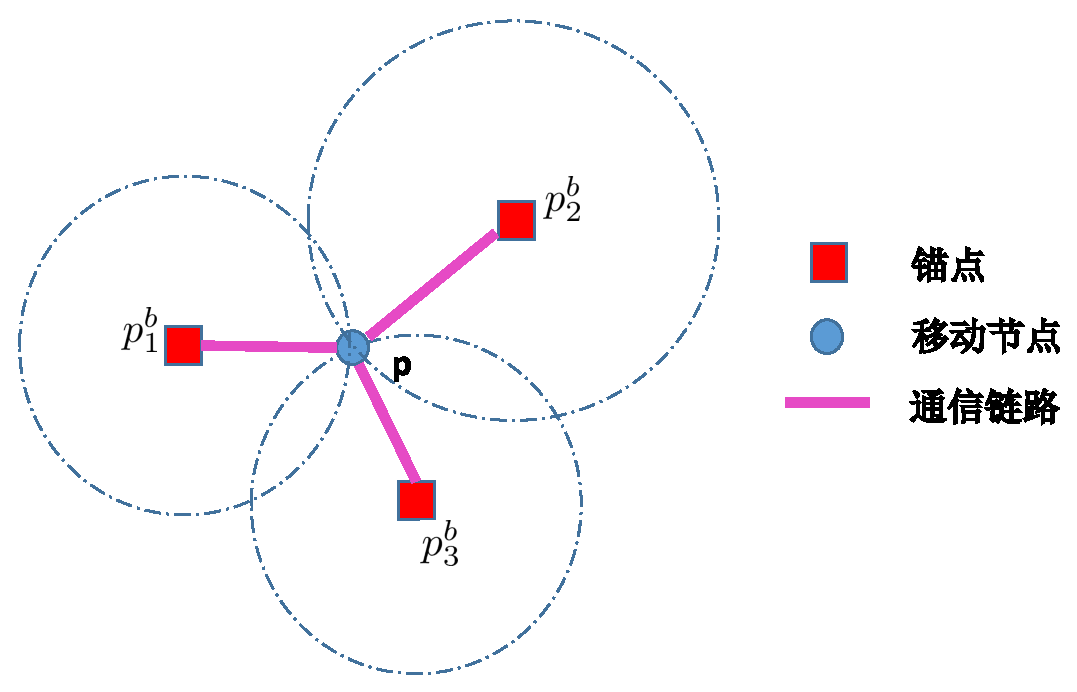
\includegraphics[width=300pt]{non_cooperative_spatial.eps}
          \caption{非协作静态场景下的定位}\label{fig:non_cooperative_spatial}
        \end{figure}
假设\textbf{待定位节点}和每一个锚点都可以相互通信进行无线测距,距离测量量服从均值为$||\bm{p}^b_i-\bm{p}||$,方差为$\sigma_i$的正态分布$X_i$。

$N_b$个\textbf{独立}测量量的联合概率分布为:
\begin{equation}\label{eq:single}
f(x_1,...x_{N_b}|\textbf{p})=\prod_{i=1}^{N_b}\frac{1}{\sqrt{2\pi\sigma_i^2}}exp\left(-\frac{(x_i-||\bm{p}^b_i-\bm{p}||)^2}{2\sigma_i^2}\right).
\end{equation}

根据点估计的理论,对于一个无偏估计量,它的方差的下界是\textbf{费舍尔信息量}(Fisher Information)的倒数,称之为\textbf{克拉美罗界}(Crame Rao Bound),在本文的讨论中,也称之为定位误差下界(Spatial Position Error Bound),它的计算公式为:
\begin{equation}\label{eq:SPEB_formula}
  \text{SPEB}=\text{tr}(\bm{I(\bm{p})}^{-1}).
\end{equation}
  % - A title should summarize the slide in an understandable fashion
  %   for anyone how does not follow everything on the slide itself.


{费舍尔信息矩阵}
以节点的\textbf{2维}位置为待估计参数,费舍尔信息量推广为\textbf{费舍尔信息矩阵}(Fisher Information Matrix)。

对于我们的模型问题,费舍尔信息矩阵有如下的形式:
\begin{equation}\label{eq:uu}
I(\bm{p})=\displaystyle\sum_{i=1}^{N_b}\frac{1}{\sigma_i^2}\bm{u}_i\bm{u}_i^{\textrm{T}}
\end{equation}
其中
\begin{equation}
\bm{u_i}=\frac{\bm{p}^b_i-\bm{p}}{||\bm{p}^b_i-\bm{p}||}.
\end{equation}


\section[协作定位场景]{协作定位场景}\label{section:cooperative_localization}

考虑一个平面定位场景中不仅部署了$N_b$个位置已知的锚点,还有$N_a$个位置未知的待定位节点,某些位置未知的节点之间可以\textbf{彼此测距},如图(\ref{fig:cooperative_spatial})所示。第i和第j个未知节点距离测量量服从均值为$||\bm{p}_i-\bm{p}_j||)$,方差为$\sigma_{ij}$的正态分布$X_{ij}$。
        \begin{figure}
          \centering
          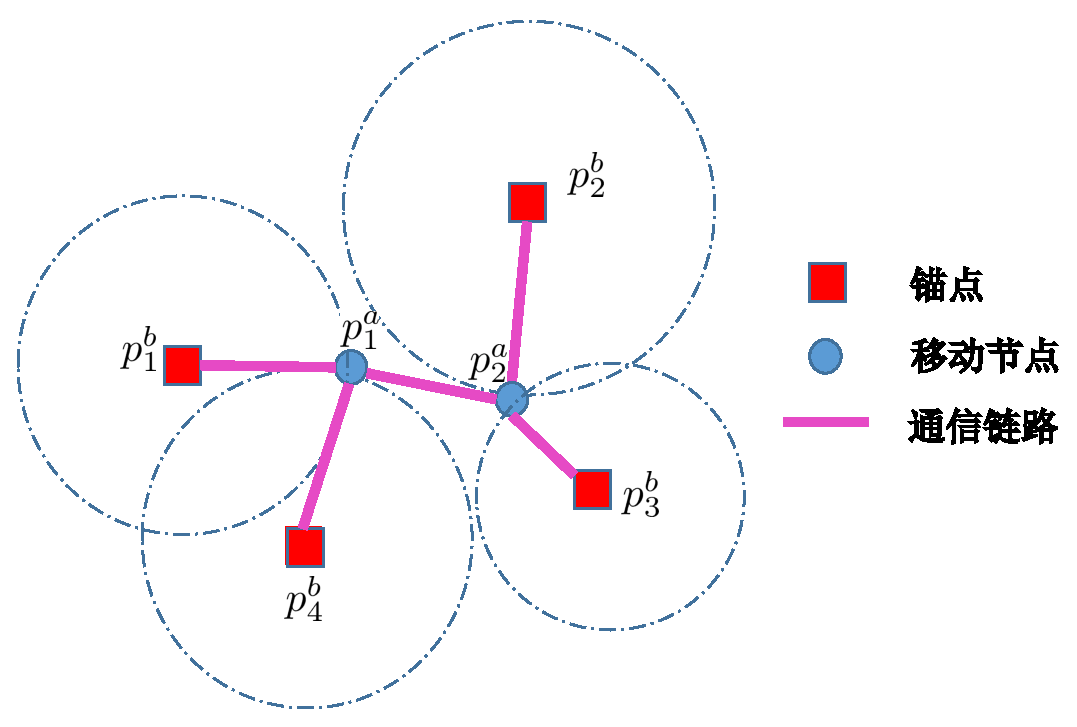
\includegraphics[width=300pt]{cooperative_spatial.eps}
          \caption{协作静态场景下的定位}\label{fig:cooperative_spatial}
        \end{figure}

以$N_a$个未知节点的位置$\{p_i\}$作为待估计的参数,可以得到测距量的联合概率密度函数为

\begin{equation}
F(\bm{X}|\bm{P})=\prod_{i=1}^{N_a} f(x^i_1,...x^{i}_{N_b}|\bm{p_i})\prod_{(i,j)\in \mathcal{E}}\frac{1}{\sqrt{2\pi\sigma_{ij}^2}}exp\left(-\frac{(x_{ij}-||\bm{p}_i-\bm{p}_j||)^2}{2\sigma_{ij}^2}\right).
\end{equation}
上式中f的具体表达式为式(\ref{eq:single}),$\mathcal{E}$表示可以彼此测距的未知节点的二元组的集合,而$x_t^i$表示第t个锚点和第i个未知节点的距离测量量。


仿照单节点时费舍尔信息矩阵的推导,关于$2N_a$个参数$\{p_i\}$的费舍尔信息矩阵$\bm{I}(\bm{P})$有如下的表达形式:
\begin{equation}\label{eq:general_fim}
\bm{I}(\bm{P})=
\left(
\begin{array}{cccc}
I(\bm{p}_1)+&-\bm{C}_{1,2}&...&-\bm{C}_{1,N_a}\\
\sum_{j\in \{1,..N_a\}\backslash\{1\}}\bm{C}_{1,j}&&&\\
&&&\\
-\bm{C}_{1,2} & I(\bm{p}_2)+
&...&-\bm{C}_{2,N_a}\\
&\sum_{j\in \{1,..N_a\}\backslash \{2\}}\bm{C}_{2,j}&&\\
&&&\\
\vdots &\vdots&\ddots &\vdots\\
&&&\\
&&&I(\bm{p}_{N_a})+\\
-\bm{C}_{1,N_a}&-\bm{C}_{2,N_a}&...& \sum_{j\in \{1,..N_a\}\backslash\{N_a\}}\bm{C}_{N_a,j}\\
\end{array}
\right).
\end{equation}
上面的式子中$I(\bm{p}_i)$表示$N_b$个锚点对未知节点距离测量的贡献,和前面的(\ref{eq:uu})式相同。$C_{i,j}=\bm{1}_{(i,j)\in E}\bm{u}_{ij}\bm{u}_{ij}^{\textrm{T}} /\sigma^2_{ij}$,表示未知节点i和j协作的矩阵。
$\bm{u}_{ij}=\frac{\bm{p}_i-\bm{p}_j}{||\bm{p}_i-\bm{p}_j||}$表示未知节点i和j的方向向量。
\section[时间协作定位]{时间协作定位}\label{section:temporal_cooperative_localization}

\subsection{单个待测节点时间协作定位}

考虑一个平面定位场景中有一个待定位的移动节点,场景中部署的$N_b$个位置已知的锚点分别在在$t_1,\dots,t_{N_a}$时刻对该节点进行定位,移动节点可以通过自身的加速度传感器对自己的速度有测量,如图(\ref{fig:cooperative_single_temporal})所示。
        \begin{figure}
          \centering
          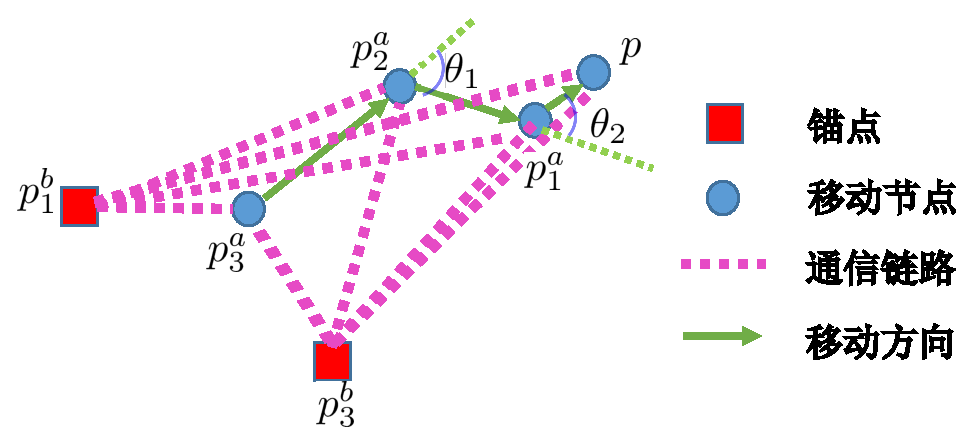
\includegraphics[width=300pt]{cooperative_single_temporal.eps}
          \caption{协作动态场景下的定位}\label{fig:cooperative_single_temporal}
        \end{figure}

假设测量时间间隔比较小使得相邻测量间节点速度方向可近似看作不变,速度测量值服从均值为$v$,方差为$\sigma_{v}$的正态分布$V_{ij}$。
那么以节点各时刻的的位置$\{p_i\}$作为待估计的参数,可以得到包括相邻时刻间的所有测距量的联合概率密度函数为
\begin{equation}
F(\bm{X}|\bm{P})=\prod_{i=1}^{N_a} f(x^i_1,...x^{i}_{N_b}|\bm{p_i})
\prod_{i=1}^{N_a-1}\frac{1}{\sqrt{2\pi}\sigma_v(t_{i+1}-t_i)}
exp\left(-\frac{(v_{i,i+1}(t_{i+1}-t_i)-||\bm{p}_i-\bm{p}_{i+1}||)^2}{2\sigma_v^2(t_{i+1}-t_i)^2}\right).
\end{equation}
费舍尔信息矩阵关于$2N_a$个参数$\{p_i\}$的费舍尔信息矩阵有如下的表达形式:
\begin{equation}\label{eq:time_cooperation_matrix}
\bm{I}(\bm{P})=
\left(
\begin{array}{ccccc}
I(\bm{p}_1)+\bm{C}_{1,2}&-\bm{C}_{1,2}&\bm{0}&\dots&\bm{0}\\
&&&&\\
-\bm{C}_{1,2} & I(\bm{p}_2)+\bm{C}_{1,2}+\bm{C}_{2,3}&-\bm{C}_{2,3}&\dots&\bm{0}\\
\vdots &\vdots&\ddots &\vdots&\vdots\\
&&&&\\
\bm{0}&\bm{0}&...& -\bm{C}_{N_a-1,N_a}&\bm{C}_{N_a-1,N_a}+I(\bm{p}_{N_a})\\
\end{array}
\right).
\end{equation}
上面的式子中若将2乘2的矩阵看作单位元素,则是一个三对角的矩阵。$I(\bm{p}_i)$表示$N_b$个锚点对未知节点距离测量的贡献,和前面的(\ref{eq:uu})式相同。$C_{i,i+1}=\bm{1}_{(i,j)\in E}\bm{u}_{ij}\bm{u}_{ij}^{\textrm{T}} /(\sigma_v^2(t_{i+1}-t_i)^2)$,表示未知节点i和j协作的矩阵,$\bm{u}_{ij}$表示未知节点i和j的方向向量。

\subsection{两个待测节点时间上一次协作}

考虑一个平面定位场景中有两个待定位的移动节点$p,q$,在初始时刻$t_1$两个移动节点之间有一次测距,服从无偏的标准差为$\sigma$的正态分布,之后时刻$t_2,\dots,t_{N_a}$两个节点不再协作,在各个时刻场景中部署的$N_b$个位置已知的锚点都可以对两个节点进行定位,移动节点可以通过自身的加速度传感器对自己的速度有测量,
假设时间间隔比较小使得相邻测量间节点速度方向可近似看作不变,速度测量值分别服从方差为$\sigma_i$的正态分布$V_i$和标准差为$\sigma'_i$的正态分布$V'_i$(均值未知,但测量是无偏的),同时假设每个节点从$t_i$到$t_{i+1}$时刻的角度符从$[0,2\pi]$的正态分布,但角度没有测量量,是未知参数。我们试图研究初始时刻$t_1$两个移动节点之间的一次测距对后续$t_n$时刻每个节点的定位精度平均来说还有多大的贡献?

针对两个节点各时刻的的位置$\{p_i,q_i\}$共计$2N_a$个二维向量作为待估计的参数,可以得到包括相邻时刻间的所有测距量的联合概率密度函数为
\begin{equation}
\begin{split}
F(\bm{X}|\bm{P})&=\frac{1}{\sqrt{2\pi\sigma^2}}exp\left(-\frac{(x-||\bm{p}_1-\bm{q}_1)^2}{2\sigma^2}\right)\prod_{i=1}^{N_a}
f(x^i_1,...x^{i}_{N_b}|\bm{p_i})
\prod_{i=1}^{N_a} f(x^i_1,...x^{i}_{N_b}|\bm{q_i})\\
&\prod_{i=1}^{N_a-1}\frac{1}{\sqrt{2\pi}\sigma_i(t_{i+1}-t_i)}
exp\left(-\frac{(v_i(t_{i+1}-t_i)-||\bm{p}_i-\bm{p}_{i+1}||)^2}{2\sigma_i^2(t_{i+1}-t_i)^2}\right)\\
&\prod_{i=1}^{N_a-1}\frac{1}{\sqrt{2\pi}\sigma'_i(t_{i+1}-t_i)}
exp\left(-\frac{(v'_i(t_{i+1}-t_i)-||\bm{q}_i-\bm{q}_{i+1}||)^2}{2\sigma^{'2}_i(t_{i+1}-t_i)^2}\right).
\end{split}
\end{equation}
我们可以将第二个模型问题与线性网络单节点时间协作建立联系,只需对上面概率密度函数中出现的符号重排即可:
将两移动节点在$t_1$时刻的协作的边作为链路的中心,该链路记为$l$,左右各有$N_a$个节点,分别表示各节点$t_i$时刻的位置。
以其中一个移动节点为参照,研究其$t_{N_a}$时刻的位置在有无$l$的影响,无$l$时,协作链路长度只有$N_a-1$,有$l$时,协作链路长度是$2N_a-1$,增加了$N_a$条链路的协作信息。于是得到的费舍尔信息矩阵与式(\ref{eq:time_cooperation_matrix})形式相同,维数为$4N_a$。

\section{本章小结}\label{section:model_discussion}
上面三小节给出了三种典型的定位场景,一般来说:
\begin{itemize}
  \item 如果测量误差$\sigma$有一个最小的阀值的话,部署的锚点不能离目标节点太近以及多个目标节点之间的距离也不能太近,否则正态分布有可能产生负的距离量,在这个限制下,于是随着网络中目标节点数目的增加,满足我们的模型的平面定位网络的覆盖范围也随之增大。
  \item 另外目标节点由于信道等原因,一般只能和距离自身比较近的其他目标节点进行通信,体现在式(\ref{eq:general_fim})描述的矩阵上即为$\bm{I}(\bm{P})$是大型稀疏矩阵。
  \item 在动态协作网络中,相邻两次测量的时间间隔$\Delta t$越小,对节点整个轨迹的追踪会更准确。但相邻两次测量的时间间隔受客观条件的限制不能无限小,研究$\Delta t \to 0$,时定位误差下界的性态只是在理论上有指导意义,实际系统无法实现。
\end{itemize}
